\documentclass[12pt,a4paper]{article}
\usepackage[english]{babel}
\usepackage[utf8]{inputenc}
\usepackage{amsmath}
\usepackage{amsfonts}
\usepackage{amssymb}
\usepackage{graphicx}
\usepackage{booktabs}
\usepackage{float}
\usepackage{hyperref}
\usepackage{xcolor}
\usepackage{listings}
\usepackage{geometry}

\geometry{a4paper, margin=2.5cm}

\title{Comparative Analysis of Sampling Methods in CMA-ES}
\author{Fernando Sampalo}
\date{\today}

\begin{document}

\maketitle

\begin{abstract}
This report presents a comparative analysis of three sampling schemes within the CMA-ES (Covariance Matrix Adaptation Evolution Strategy) algorithm: classical Gaussian sampling, Sobol sequences, and Latin Hypercube sampling. The methods are evaluated on a diverse set of standard optimization benchmarks, analyzing performance in terms of convergence, accuracy, and runtime. The results show substantial differences between methods, with practical implications for choosing sampling strategies in real-world optimization.
\end{abstract}

\section{Practical notes}
\begin{itemize}
    \item Running the accompanying code typically takes about two minutes.
    \item GitHub repository (contributions welcome): \url{https://github.com/fsampalo/Experimentacion-CMA-ES}
\end{itemize}


\section{Introduction}
CMA-ES is an evolutionary optimization algorithm that has proved particularly effective for continuous black-box problems. A key design choice is how candidate solutions are sampled. This study compares three sampling approaches, each with distinct properties and potential advantages.

\section{Sampling methods}

\subsection{Classical Gaussian sampling}
Classical Gaussian sampling is the traditional choice in CMA-ES. Candidates are drawn from a multivariate normal distribution whose covariance matrix is adapted during the search. Its main features are:
\begin{itemize}
    \item Perturbations follow a normal distribution
    \item Covariance adaptation driven by selection
    \item Exploration via random perturbations in search space
\end{itemize}

\subsection{Sobol sequence}
The Sobol sequence is a low-discrepancy quasi-random construction that tends to cover the domain more evenly than plain random sampling. Notable properties include:
\begin{itemize}
    \item Deterministic point generation (for a fixed counter state)
    \item More uniform spatial spread than i.i.d.\ random sampling
    \item Often lower variance in Monte Carlo-style estimates
\end{itemize}

\subsection{Latin Hypercube}
Latin Hypercube sampling stratifies each coordinate axis and draws one sample per stratum, improving marginal coverage. Benefits include:
\begin{itemize}
    \item Better coverage of the search space
    \item Reduced correlation across dimensions compared with naive random sampling
    \item Efficient exploration in many practical settings
\end{itemize}

\section{Experimental setup}

\subsection{Parameters}
\begin{itemize}
    \item Problem dimension: 10 (8 for the Powell function, which requires a multiple of four)
    \item Population size: 50
    \item Maximum iterations: 100
    \item Independent runs: 30 per method--function pair
    \item Search domain: $[-5, 5]$ in every coordinate
\end{itemize}

\subsection{Benchmark functions}
The following test functions were used:
\begin{itemize}
    \item Sphere (simple convex bowl)
    \item Rosenbrock (curved valley)
    \item Rastrigin (many local minima)
    \item Ackley (high-frequency ripples)
    \item Schwefel (misleading landscape)
    \item Griewank (many suboptimal peaks)
    \item Levy (multimodal)
    \item Zakharov (quadratic with coupling)
    \item Dixon--Price (sensitive to scaling)
    \item Powell (ill-conditioned)
    \item Sum-Squares (weighted quadratic)
    \item Trid (quadratic interactions)
\end{itemize}

\section{Results and analysis}

\subsection{Convergence behaviour}
Overall, the sampling schemes differ markedly in how quickly they improve the best objective value:
\begin{itemize}
    \item \textbf{Gaussian sampling} is more erratic and can escape shallow local structure, but in our experiments it most often achieved the weakest final values and required more iterations to reach comparable accuracy.
    \item \textbf{Sobol sampling} yielded the most stable and predictable improvement and, on average, the tightest final objectives. This supports the idea that low-discrepancy normal variates can be effective inside CMA-ES-style updates.
    \item \textbf{Latin Hypercube} offers a good compromise between exploration and exploitation: final qualities were often close to Sobol, though convergence sometimes needed more iterations.
\end{itemize}

Below we highlight a few representative runs; full comparison plots are under \texttt{imgs/comparisons}:

\begin{figure}[H]
    \centering
    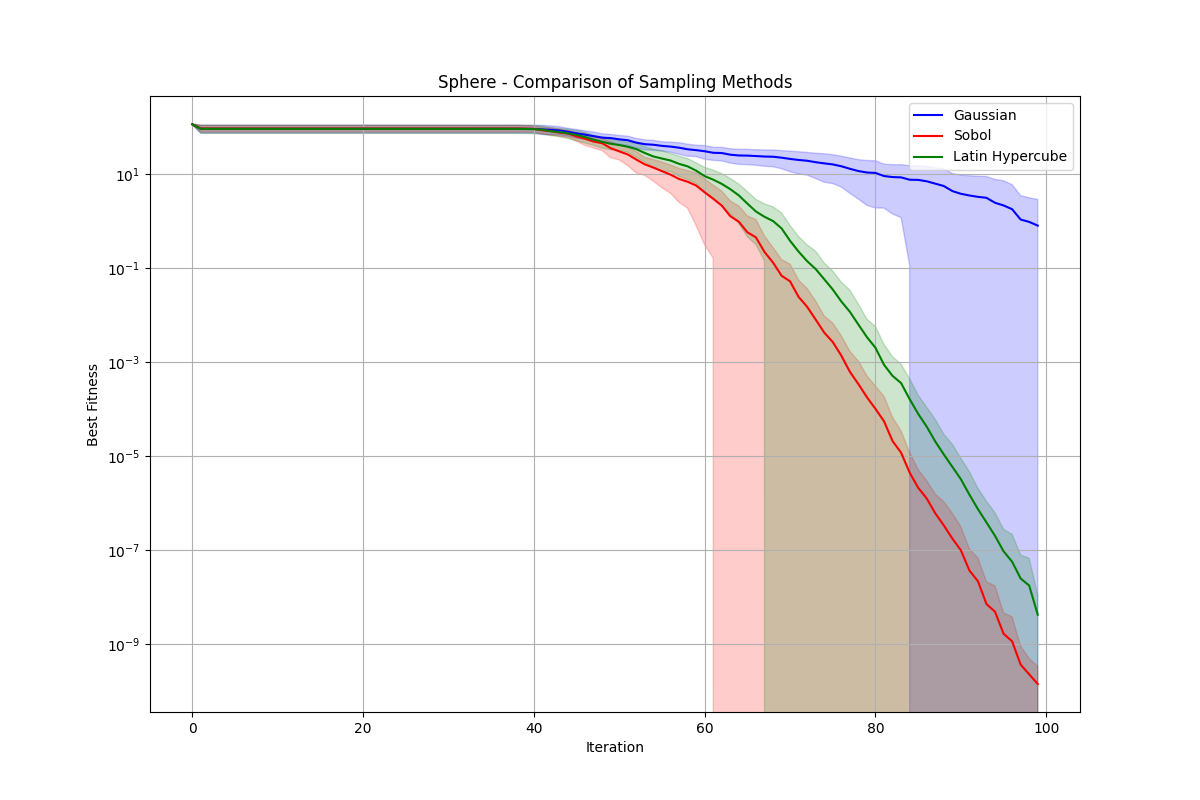
\includegraphics[width=0.8\textwidth]{imgs/comparisons/Sphere_comparison.png}
    \caption{Convergence comparison on the Sphere function}
    \label{fig:sphere}
\end{figure}

Figure~\ref{fig:sphere} shows Sobol and Latin Hypercube reaching similar best values, whereas Gaussian sampling does not reach equally accurate solutions within the same iteration budget.


\begin{figure}[H]
    \centering
    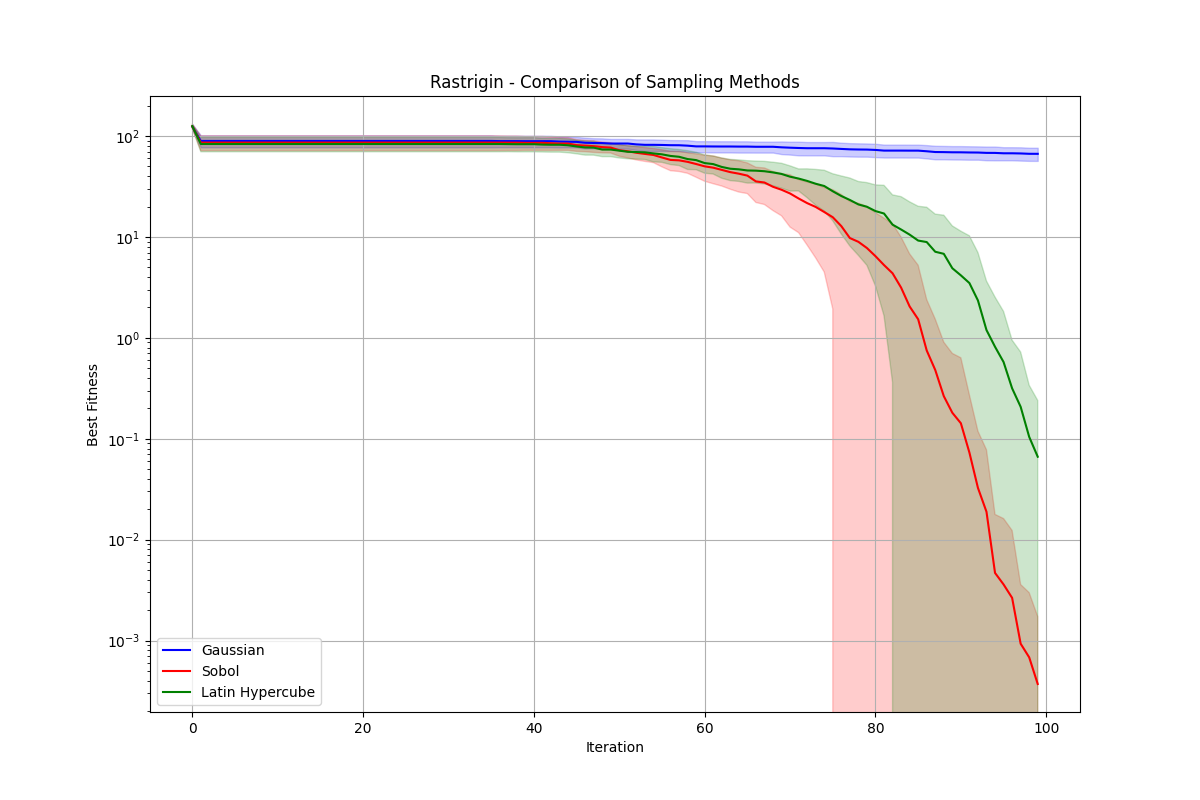
\includegraphics[width=0.8\textwidth]{imgs/comparisons/Rastrigin_comparison.png}
    \caption{Convergence comparison on the Rastrigin function}
    \label{fig:rastrigin}
\end{figure}

Figure~\ref{fig:rastrigin} again shows Sobol and Latin Hypercube performing comparably, in contrast to Gaussian sampling, which improves more slowly.

\begin{figure}[H]
    \centering
    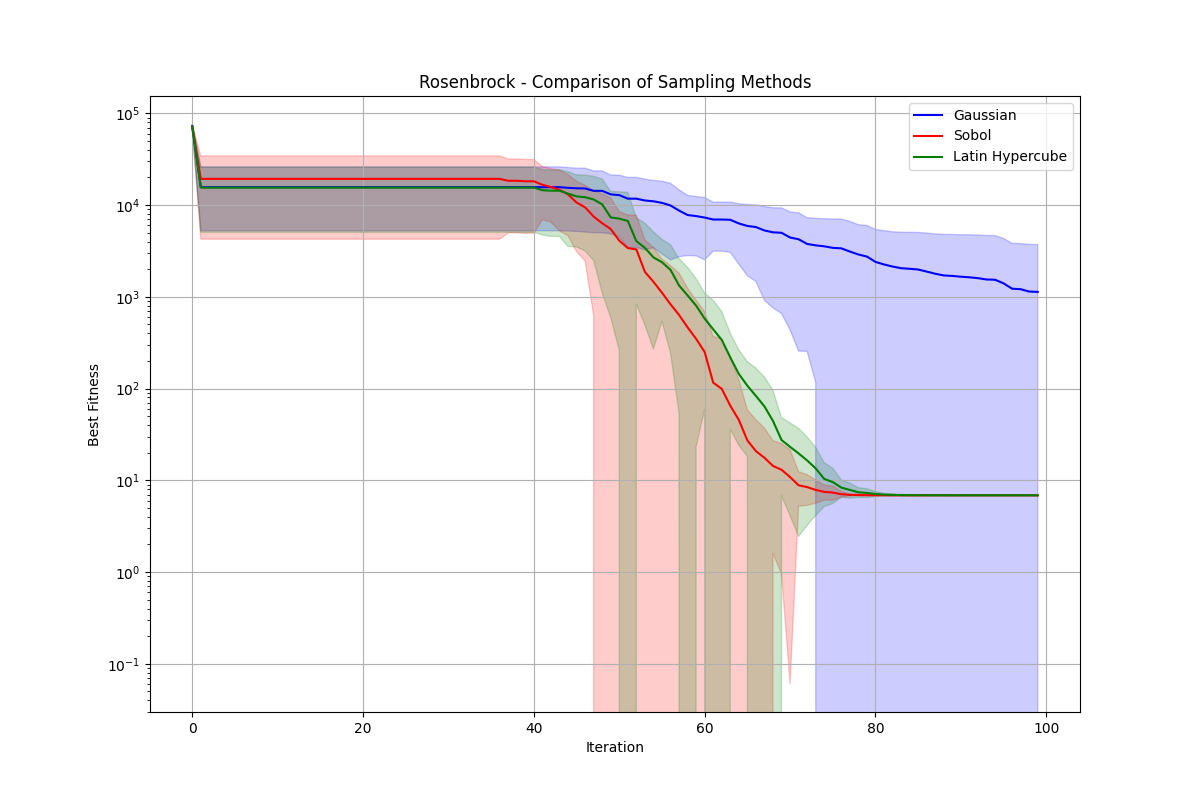
\includegraphics[width=0.8\textwidth]{imgs/comparisons/Rosenbrock_comparison.png}
    \caption{Convergence comparison on the Rosenbrock function}
    \label{fig:rosenbrock}
\end{figure}

As in Figure~\ref{fig:rosenbrock}, Sobol and Latin Hypercube behave similarly, while Gaussian sampling is less sample-efficient in early iterations.

\begin{figure}[H]
    \centering
    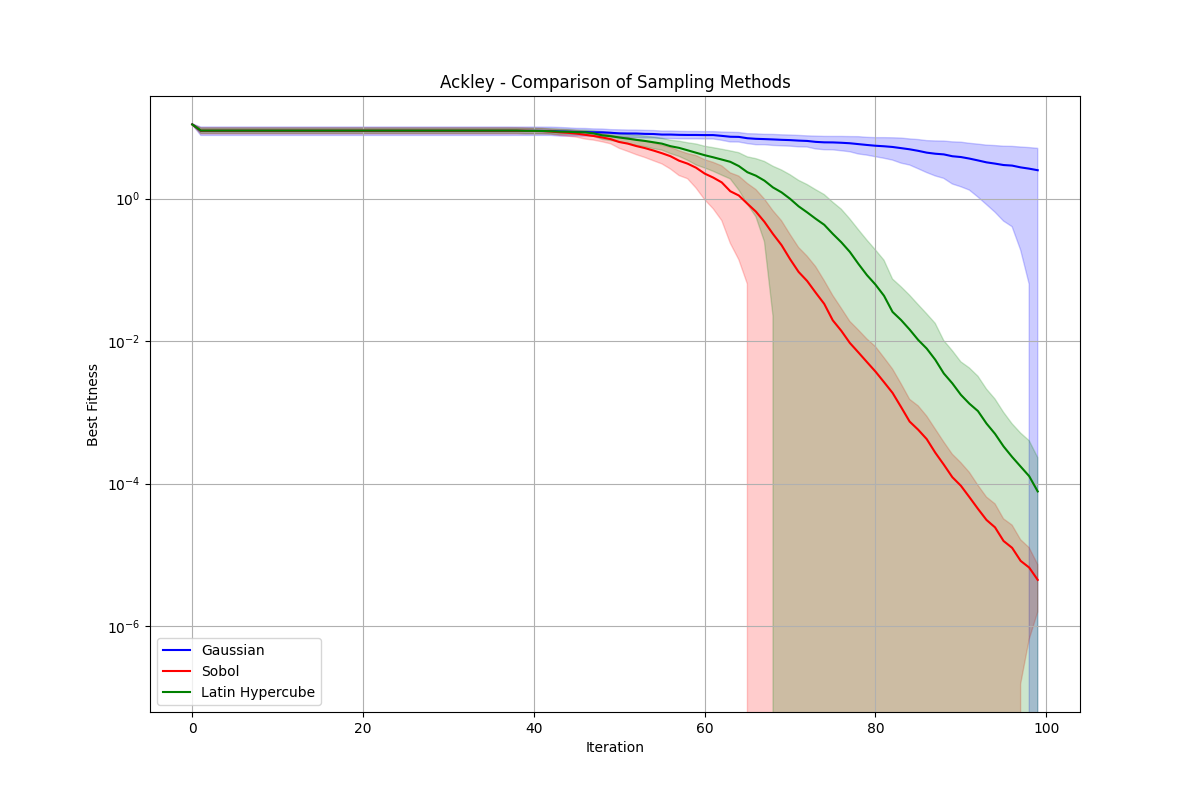
\includegraphics[width=0.8\textwidth]{imgs/comparisons/Ackley_comparison.png}
    \caption{Convergence comparison on the Ackley function}
    \label{fig:ackley}
\end{figure}

Figure~\ref{fig:ackley} highlights comparable performance for Sobol and Latin Hypercube, with Gaussian sampling initially lagging in accuracy.

\begin{figure}[H]
    \centering
    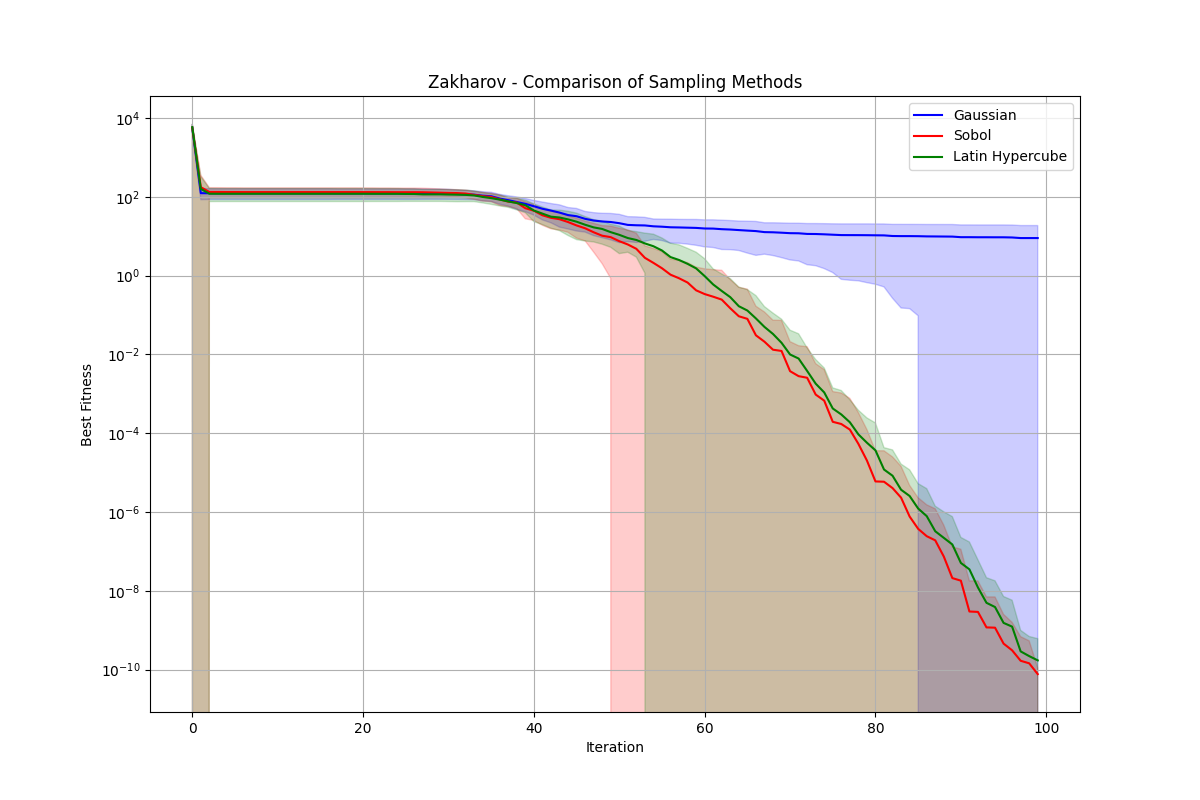
\includegraphics[width=0.8\textwidth]{imgs/comparisons/Zakharov_comparison.png}
    \caption{Convergence comparison on the Zakharov function}
    \label{fig:zakharov}
\end{figure}

Figure~\ref{fig:zakharov} shows Sobol and Latin Hypercube converging at a similar rate, whereas Gaussian sampling needs more iterations for comparable precision.

\subsection{Statistical testing}
Pairwise Mann--Whitney $U$ tests were applied to final fitness values across runs:

\begin{table}[H]
    \centering
    \begin{tabular}{lccc}
        \toprule
        Function & Gaussian vs Sobol & Gaussian vs LHC & Sobol vs LHC \\
        \midrule
        Sphere & $0.0001$ & $0.0001$ & 0.7845 \\
        Rosenbrock & $0.0001$ & $0.0001$ & 0.4119 \\
        Rastrigin & $0.0001$ & $0.0001$ & $0.0001$ \\
        Ackley & $0.0001$ & $0.0001$ & $0.0001$ \\
        Schwefel & 0.3545 & 0.0001 & 0.0001 \\
        \bottomrule
    \end{tabular}
    \caption{$p$-values from Mann--Whitney $U$ tests (subset of benchmarks)}
    \label{tab:stats}
\end{table}

We find strong evidence ($p < 0.0001$) of differences between Gaussian vs.\ Sobol and Gaussian vs.\ LHC for the listed functions, and between Sobol vs.\ LHC for Rastrigin, Ackley, and Schwefel. Differences between Sobol and LHC are not significant for Sphere ($p = 0.7845$) or Rosenbrock ($p = 0.4119$).

\subsection{Runtime}
\begin{itemize}
    \item Gaussian sampling is usually the fastest per iteration
    \item Sobol sequences incur higher overhead
    \item Latin Hypercube sits in between
\end{itemize}

\begin{figure}[H]
    \centering
    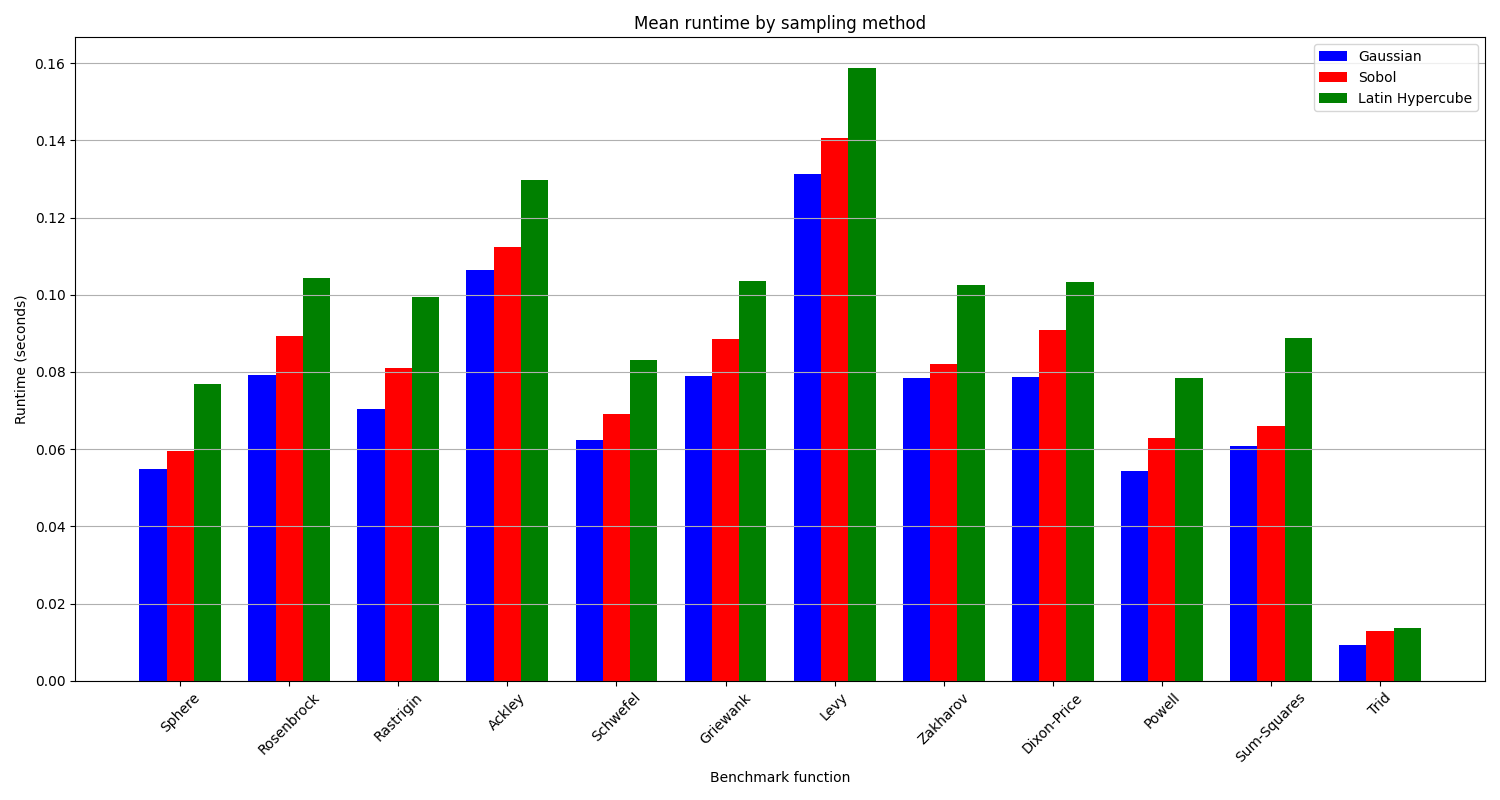
\includegraphics[width=0.8\textwidth]{imgs/comparisons/runtime_comparison.png}
    \caption{Runtime comparison across sampling methods}
    \label{fig:runtime}
\end{figure}

\section{Discussion}
Method choice should reflect:
\begin{itemize}
    \item Problem structure (multimodality, conditioning, noise)
    \item Computational budget
    \item Whether wide exploration or fast local refinement is more important
\end{itemize}

If wall-clock speed is secondary to solution quality, Sobol and Latin Hypercube sampling are preferable in our benchmark suite.

\section{Conclusions}
\begin{itemize}
    \item No single sampling rule is universally best; in our runs Sobol most often reached high-quality minima in fewer iterations.
    \item Sobol and Latin Hypercube excel on harder landscapes where coverage matters.
    \item Gaussian sampling remains simple and fast per step, but may require many more iterations on difficult functions.
\end{itemize}

\section{Future work}
Possible extensions include:
\begin{itemize}
    \item Hybrid sampling schedules
    \item Adapting the sampler during the run
    \item Scaling studies in higher dimensions
    \item Case studies on real engineering or ML hyperparameter tasks
    \item Additional diversification mechanisms for highly multimodal objectives
\end{itemize}

\end{document}
